% Intended LaTeX compiler: pdflatex
\documentclass[10pt,a4paper,UTF8]{article}
\usepackage{zclorg}
\author{张朝龙}
\date{}
\title{练习:线性映射}
\hypersetup{
 pdfauthor={张朝龙},
 pdftitle={练习:线性映射},
 pdfkeywords={},
 pdfsubject={},
 pdfcreator={Emacs 25.0.50.1 (Org mode 9.0.5)}, 
 pdflang={English}}
\begin{document}

\maketitle
\tableofcontents
\titlepic{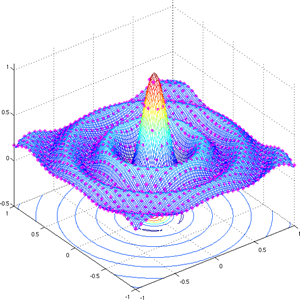
\includegraphics[scale=0.25]{../../img/sinc.PNG}}

\section{3.A.1}
\label{sec:org64409a6}


\begin{problem}
设\(b,c\in  \mathbf{R}\),定义\(T: \mathbf{R}^{3} \rightarrow \mathbf{R}^{2}\) 如下:
\[T(x,y,z) = (2x-4y+3z +b,6x+cxyz)\]
证明\(T\)是线性的当且仅当\(b=c=0\)
\end{problem}

\begin{answer}
首先:如果\(T\)是线性的,必有\(T(0) = 0\),从而有\((b,0) = (0,0)\),即\(b=0\)。

另外有\(T(1,1,1) = T(1,1,0) + T(0,0,1)\),推出\((1+b,6+c) = (-2+b,6) + (3+b,0)\),即有\(c+0\)

接下来证明\(b=c=0\)所以\(T\)是线性的。因为\(b=c=0\),则\(T\)可以写成:
\[T(x,y,z) = (2x-4y+3z,6x)\]
这个映射是如下线性映射的特例。

从\(\mathbf{F}^{n}\)到\(\mathbf{F}^{m}\),设\(m,n\)是正整数,\(A_{j,k}\in \mathbf{F},j = 1,\ldots ,m,k=1,\ldots ,n\),定义\(T\in \mathcal{L}(\mathbf{F}^{n}, \mathbf{F}^{m})\)为:
\begin{equation}
\label{eq:201704033}
T(x_{1},x_{2},\ldots ,x_{n}) = (A_{1,1}x_{1} + \ldots  + A_{1,n}x_{n}, \ldots , A_{m,1}x_{1} + \ldots + A_{m,n}x_{n})
\end{equation}
式\ref{eq:201704033}可以写成矩阵的形式为:
\begin{equation}
\label{eq:201704034}
\begin{bmatrix}
y_{1} \\ y_{2} \\ \vdots \\ y_{m}
\end{bmatrix}
=
\begin{bmatrix}
A_{1,1} & A_{1,2}  & \ldots & A_{1,n} \\
A_{2,1} & A_{2,2}  & \ldots & A_{2,n} \\
\vdots & \vdots  & \ddots & \vdots \\
A_{m,1} & A_{m,2}  & \ldots & A_{m,n} \\
\end{bmatrix}
\begin{bmatrix}
x_{1} \\ x_{2} \\ \vdots \\ x_{n}
\end{bmatrix}
\end{equation}
\end{answer}
\section{3.A.2}
\label{sec:orgaa1fe74}


\begin{problem}
设\(b,c\in \mathbf{R}\),定义\(T: \mathcal{P}( \mathbf{R}) \rightarrow \mathbf{R}^{2}\)如下:
\begin{equation}
\label{eq:1}
Tp = (3p(4) + 5p^{'}(6) + bp(1)p(2),\int_{-1}^{2}x^{3}p(x)dx + c\sin p(0))
\end{equation}
证明\(T\)是线性的当且仅当\(b=c=0\)
\end{problem}

\begin{answer}
假设\(p,q\in \mathcal{P}(R)\),若\(T\)是线性映射则有:
\[T(p + q) = Tp + Tq\]
把(\ref{eq:1})带入上式,可得\(b=c=0\)

然后证明假设\(b=c=0\) ,\(T\)是线性映射。按照线性映射的定义来。把定义附在下面,证明过程略。

\begin{definition}
从\(V\) 到\(W\)的线性映射是具有以下性质的函数\(T: V \rightarrow W\):

加性: 对所有\(u,v \in V\)都有 \(T(u+v) = T(u) + T(v)\)

齐次: 对所有的 \(\lambda \in \mathbf{F}\) 和\(v\in V\) 都有 \(T(\lambda v) = \lambda (Tv)\)
\end{definition}
\end{answer}
\section{3.A.3}
\label{sec:orgeb03743}


\begin{problem}
设\(T\in \mathcal{L}( \mathbf{F}^{n}, \mathbf{F}^{m})\),证明存在标量\(A_{j,k},j=1,\ldots ,m,k=1,\ldots ,n\)使得对任意\(x_{1},\ldots ,x_{n}\in \mathbf{F}^{n}\)都有

\begin{equation}
\label{eq:2}
T(x_{1},\ldots ,x_{n}) = (A_{1,1}x_{1} + \ldots A_{1,n}x_{n} ,\ldots ,A_{m,1}x_{1} + \ldots +A_{m,n}x_{n})
\end{equation}
\end{problem}

\begin{answer}
我们这里准备提前使用一下矩阵的概念。

\begin{equation}
\label{eq:3}
T(x_{1},x_{2},\ldots ,x_{n}) = (A_{1,1}x_{1} + \ldots  + A_{1,n}x_{n}, \ldots , A_{m,1}x_{1} + \ldots + A_{m,n}x_{n})
\end{equation}


式\ref{eq:3}可以写成矩阵的形式为:
\begin{equation}
\label{eq:4}
\begin{bmatrix}
y_{1} \\ y_{2} \\ \vdots \\ y_{m}
\end{bmatrix}
=
\begin{bmatrix}
A_{1,1} & A_{1,2}  & \ldots & A_{1,n} \\
A_{2,1} & A_{2,2}  & \ldots & A_{2,n} \\
\vdots & \vdots  & \ddots & \vdots \\
A_{m,1} & A_{m,2}  & \ldots & A_{m,n} \\
\end{bmatrix}
\begin{bmatrix}
x_{1} \\ x_{2} \\ \vdots \\ x_{n}
\end{bmatrix}
\end{equation}
令:
\begin{equation}
\label{eq:7}
\mathbf{y} = 
\begin{bmatrix}
y_{1} \\ y_{2} \\ \vdots \\ y_{m}
\end{bmatrix}
\end{equation}
\begin{equation}
\label{eq:5}
\mathbf{A} = 
\begin{bmatrix}
A_{1,1} & A_{1,2}  & \ldots & A_{1,n} \\
A_{2,1} & A_{2,2}  & \ldots & A_{2,n} \\
\vdots & \vdots  & \ddots & \vdots \\
A_{m,1} & A_{m,2}  & \ldots & A_{m,n} \\
\end{bmatrix}
\end{equation}
\begin{equation}
\label{eq:6}
\mathbf{x} = 
\begin{bmatrix}
x_{1} \\ x_{2} \\ \vdots \\ x_{n}
\end{bmatrix}
\end{equation}

则有\(\mathbf{y} = \mathbf{Ax}\)

进而\(\mathbf{y_{1} + y_{2}} = \mathbf{A(x_{1} + x_{2})}\)
\end{answer}

\section{3.A.4}
\label{sec:org779eb8a}


\begin{problem}
设\(T\in \mathcal{L}(V,W)\)  且\(v_{1},\ldots ,v_{m}\)是\(V\)中的向量组,使得\(Tv_{1},\ldots ,Tv_{m}\)在\(W\)中是线性无关的,证明\(v_{1},\ldots ,v_{m}\)是线性无关的。
\end{problem}

\begin{answer}
假设存在\(a_{i}\in \mathbf{F},i=1,\ldots ,m\)使得:
\begin{equation}
\label{eq:8}
a_{1}v_{1} + \ldots + a_{m}v_{m} = 0
\end{equation}
则对两边使用线性映射:
\begin{equation}
\label{eq:9}
T(a_{1}v_{1} + \ldots + a_{m}v_{m}) = T(0)=0
\end{equation}
根据线性映射的齐次可加性有:
\begin{equation}
\label{eq:10}
a_{1} T(v_{1}) + \ldots + a_{m}T(v_{m}) = 0
\end{equation}

因为\(T(v_{1}),\ldots ,T(v_{m})\)是线性无关的,所以有\(a_{i} = 0,i=1,\ldots ,m\)

即证明了\(v_{1},\ldots ,v_{m}\)是线性无关的。
\end{answer}
\section{3.A.7}
\label{sec:orgdea8748}


\begin{problem}
证明每个从一维向量空间到其自身的线性映射都是乘以某个标量。准确的说,证明:若\(\dim V = 1\)且\(T\in \mathcal{L}(V,V)\),则有\(\lambda \in \mathbf{F}\)使得对所有\(v\in V\)都有\(Tv = \lambda v\)
\end{problem}

\begin{answer}
因为\(\dim V = 1\),说明\(V\)的基只有一个向量,即\(V\)中的任何一个向量都可以写成另一个非零向量的标量形式,即\(Tu = au\)。

现在考虑特定的 \(v\in V,v = bu\),则有:
\begin{eqnarray*}
Tv&=&T(bu) \\
&=&bT(u) \\
&=&bau \\
&=&abu\\
&=&av
\end{eqnarray*}
\end{answer}
\section{3.A.8}
\label{sec:orgc976621}


\begin{problem}
给出一个函数\(\phi: \mathbf{R}^{2} \rightarrow \mathbf{R}\)使得对于所有\(a\in \mathbf{R}\)和所有的\(v\in \mathbf{R}^{2}\)有:
\begin{equation}
\label{eq:11}
\phi(av) = a(\phi(v))
\end{equation}
但是\(\phi\)不是线性的。
\end{problem}

\begin{answer}
令\(\phi(x,y) = \sqrt[3]{x^{3} + y^{3}}\) 。

这个函数满足齐次性,对于\(\phi(\lambda(x,y))\),有:
\begin{eqnarray*}
\phi(\lambda x,\lambda y) &=& \sqrt[3]{(\lambda x)^{3} + (\lambda y)^{3}}  \\
&=& \lambda  \sqrt[3]{x^{3} + y^{3}}  \\ 
&=& \lambda \phi (x,y)
\end{eqnarray*}
即\(\phi\)满足齐次性。但是\(\phi\)不满足可加性,即
\begin{eqnarray*}
\phi(x_{1}+x_{2},y_{1}+y_{2})&\neq& \phi(x_{1},y_{1}) + \phi(x_{2},y_{2}) \\
\end{eqnarray*}
\end{answer}

\section{3.A.9}
\label{sec:org6b19e69}


\begin{problem}
给出一个函数\(\varphi: \mathbf{C}\rightarrow \mathbf{C}\),使得对于所有的\(w,z\in C\)都有:
\begin{equation}
\label{eq:13}
\varphi(w+z) = \varphi(w) + \varphi(z)
\end{equation}
但是\(\varphi\)不是线性的。
\end{problem}

\begin{answer}
想到了\(\varphi(z) = \Re(z)\)满足
\begin{equation}
\label{eq:14}
\varphi(u+v) = \varphi(u) + \varphi(v)
\end{equation}
但是对于\(i\in \mathbf{F}\),有:
\begin{equation}
\label{eq:15}
\varphi(i u) \neq i\varphi(u)
\end{equation}

这个问题在复数域上很好证明,但是在实数域上暂时还没有想到什么好办法。因为实数域上的加法和标量乘法是等效的,即\(\lambda u = \underbrace{u+\ldots +u}_{\lambda}\)
\end{answer}

\section{3.A.10}
\label{sec:org6eeb9c0}


\begin{problem}
设\(U\)是\(V\)的子空间且\(U\neq V\),设\(S\in \mathcal{L}(V,W)\)且\(S\neq 0\),定义\(T:V\rightarrow W\)如下:
\begin{equation}
\label{eq:16}
Tv = 
\begin{cases}
Sv & v\in U \\
0 & v\in V, v\notin U
\end{cases}
\end{equation}
证明\(T\)不是\(V\)上的线性映射。
\end{problem}

\begin{answer}
首先我们选择\(u\in U\)满足\(Su\neq 0\),然后选择\(v\in V\)使得\(v\notin U\),那么肯定有\(u+v\notin U\)

不然的话就会有\(v = (u+v) - u \in U\),产生矛盾。因此\(u+v\notin U\). 又因为\(u\in U\),且\(U\)是\(V\)的子空间,所以\(u\in V\),所以\(u+v \in V\),综上有\(u+v \in V\) \(u+v \notin U\)

那么有\(T(u+v) = 0\),但是\(Tu + Tv = Su + 0 \neq 0\),所以\(T\)不满足可加性。即\(T\)不是线性映射
\end{answer}


\section{3.A.11}
\label{sec:org5f6e9c6}


\begin{problem}
设\(V\)是有限维的。证明\(V\)的子空间上的线性映射可以扩张成\(V\)上的线性映射。也就是说,证明如果\(U\)是\(V\)的子空间,\(S\in \mathcal{L}(U,W)\),那么存在\(T\in \mathcal{L}(V,W)\)使得对于所有的\(u\in U\)都有\(Tu = Su\)
\end{problem}

\begin{answer}
首先因为\(U\)是\(V\)的子空间,\(\dim U \leq \dim V\),我们可以找到\(U\)的一个基\(\mathcal{U}\),通过对\(\mathcal{U}\)扩展\(\dim V-\dim U\)个线性无关组,我们可以得到\(V\)的一个基\(\mathcal{V}\)。所以根据3.5存在一个唯一的线性映射\(T:V\rightarrow W\),并且满足:
\begin{equation}
\label{eq:12}
Tu_{i} = Su_{i},Tv_{i} = 0
\end{equation}
其中\(i\in \{1,\ldots ,\dim U\}\),\(j\in \{\dim U +1,\ldots ,\dim V\}\)

对于所有的\(u = a_{1}u_{1} + \ldots + a_{\dim U}u_{\dim U} , a_{i}\in \mathbf{F}\),有:
\begin{eqnarray}
\label{eq:17}
Tu&=&T(a_{1}u_{1} + \ldots + a_{\dim U}u_{\dim U}) \\
&=&a_{1}T(u_{1}) + \ldots + a_{\dim U}T(u_{\dim U}) \\
&=&a_{1}S(u_{1}) + \ldots + a_{\dim U}S(u_{\dim U}) \\
&=&S(a_{1}u_{1} + \ldots + a_{\dim U}u_{\dim U}) \\
&=&Su
\end{eqnarray}
\end{answer}

\section{3.A.12}
\label{sec:org26708e1}


\begin{problem}
设\(V\) 是有限维的且\(\dim V > 0\),再设\(W\)是无限维的,证明\(\mathcal{L}(V,W)\)是无限维的。
\end{problem}

\begin{answer}
关于无限维空间我们之前做过一个证明:\(V\)是无限维的当且仅当\(V\)中存在一个向量序列\(v_{1},\ldots ,v_{m}\)使得当\(m\)是任意整数时\(v_{1},\ldots ,v_{m}\)都是线性无关的。

在这里我们令\(U= \mathcal{L}(V,W)\),即\(U\)是所有从\(V\)到\(W\)的线性映射的集合。由于\(W\)是无限维的,所以在\(W\)中存在\(w_{i},w_{2},\ldots\)向量组使得对于任何的\(m\)都有\(w_{1},\ldots ,w_{m}\)是线性独立的。

接下来定义\(T_{i}\in \{V,W\}\)满足\(T_{i}(v_{1}) = w_{i}\). \(T_{i}\)保证存在,但是不一定唯一。我们接下来证明对任意\(m\)都有\(T_{i}\)是线性独立的。

假设\(\exists a_{i}\in \mathbf{F},i=1,\ldots ,m\) ,满足:
\begin{equation}
\label{eq:18}
a_{1}T_{1} + \ldots + a_{m}T_{m} = 0
\end{equation}
则有:
\begin{equation}
\label{eq:19}
(a_{1}T_{1} + \ldots + a_{m}T_{m})(v_{1}) = 0
\end{equation}
因为\(0\)映射,映射所有的元素到\(0\). 接着式(\ref{eq:19}),推导,我们有:
\begin{equation}
\label{eq:20}
a_{1}(T_{1}v_{1}) + \ldots + a_{m}(T_{m}v_{1}) = 0
\end{equation}
因为\(T_{i}(v_{1}) = w_{i}\),所以:
\begin{equation}
\label{eq:21}
a_{1}w_{1} + \ldots + a_{m}w_{m}= 0
\end{equation}
因为\(w_{i}\)是线性无关的,所以有\(a_{i}=0,i=\{1,\ldots ,m\}\)

结合式(\ref{eq:18})我们有:\(T_{i},\ldots ,T_{m}\)是线性独立的。因为\(m\)是我们选的任意整数,则有\(\mathcal{L}(V,W)\)是无限维的。

通过这个题目和上一个题目在处理线性映射空间上的映射时需要把3.5的证明过程烂熟于心啊。要能够构造一些映射关系。
\end{answer}

\section{3.A.13}
\label{sec:org6352880}


\begin{problem}
设\(v_{1},\ldots ,v_{m}\)是\(V\)中的一个线性相关向量组,并设\(W\neq 0\),证明存在\(w_{1},\ldots ,w_{m}\in W\)使得没有\(T\in \mathcal{L}(V,W)\)满足\(Tv_{k} = w_{k},k=1,\ldots ,m\)
\end{problem}

\begin{answer}
我们采用3.A.11,3.A.12类似的方法,构造一个映射不是线性的即可。

因为\(W\neq 0\),所以我们可以定义\(T:V\rightarrow W\),使得:
\begin{equation}
\label{eq:22}
T(a_{1}v_{1} + \ldots + a_{m}v_{m}) = a_{1}w_{1} + \ldots + a_{m}w_{m}, w_{j}\neq 0
\end{equation}
又因为\(v_{1},\ldots ,v_{m}\)是线性相关的所以存在不全为零的\(b_{i},i=1,\ldots ,m\)使得:
\begin{equation}
\label{eq:23}
b_{1}v_{1} + \ldots + b_{m}v_{m} = 0
\end{equation}
则有:
\begin{equation}
\label{eq:24}
T(b_{1}v_{1} + \ldots + b_{m}v_{m}) = 0
\end{equation}
根据\(T\)的定义:
\begin{equation}
\label{eq:25}
T(b_{1}v_{1} + \ldots + b_{m}v_{m}) = b_{1}w_{1} + \ldots + b_{m}w_{m}
\end{equation}
又因为\(w_{j}\neq 0\),式(\ref{eq:23})和式(\req{eq:24})矛盾。因此\(T\)不是线性映射。
\end{answer}

\section{3.A.14}
\label{sec:orgb67a255}


\begin{problem}
设\(V\)是有限维的且\(\dim V \geq 2\).证明存在\(S,T\in \mathcal{L}(V,V)\)使得\(ST\neq TS\)
\end{problem}

\begin{answer}
假设\(e_{1},\ldots ,e_{n}\)是\(V\)的一组基\(\dim V = n\),定义\(T\in \mathcal{L}(V,V)\)满足:
\begin{equation}
\label{eq:26}
Te_{1} = e_{2}, Te_{2} = e_{1}, Te_{i} = e_{i}, i > 2
\end{equation}
定义\(S\in  \mathcal{L}(V,V)\)满足:
\begin{equation}
\label{eq:27}
Se_{1} = e_{1}, Se_{2} = 2 e_{2}, Se_{i} = e_{i}, i > 2
\end{equation}

则有\(TS(e_{1}) = e_{2},TS(e_{2}) = 2e_{1}\) \(ST(e_{1}) = 2e_{2},ST(e_{2}) = 2e_{1}\)

\(TSe_{1} \neq STe_{1}\)
\end{answer}
\end{document}
